\chapter{基于KAN的知识融合因果发现方法研究}
识别特征间的因果关系是当前人工智能可解释性发展的核心目标之一，也是制定基于证据的可靠决策的重要前提。然而，当前因果研究领域的多数工作仍集中于识别变量间是否存在因果关系、构建因果图的拓扑结构，对原因如何定量影响结果的映射关系缺乏深入探索。学习因果映射表示，本质上是揭示因果关系的定量作用规律，这一目标的实现，不仅能深化对因果机制的理解，将因果发现从“存在性判断”推向“作用机制解析”，更能增强因果模型的可解释性，使模型输出的因果关系具备明确的物理意义或实际应用价值。针对这一研究缺口，本文提出Causal-KAN框架，通过将领域内的因果知识以结构化方式嵌入柯尔莫哥洛夫-阿诺特网络（KANs），实现因果映射表示的精准学习。该框架的核心目标在于突破传统神经网络在建模结构因果模型（SCMs）时的固有局限性：传统深度学习模型（如多层感知器）虽具备强大的函数逼近能力，但复杂的网络结构导致因果关系被黑箱架构所掩盖，既无法明确因果作用的具体路径，也难以与领域先验知识有效融合。为达成这一目标，本研究提出两项关键创新：(1) 设计与KAN架构原生兼容的知识融合方法，将已知的因果关系（如父节点集合、边方向）转化为网络的结构性约束，显式建模SCMs中的结构函数$f_i$，避免非因果变量的干扰；(2) 借助针对性的初始化方案与掩码约束机制，实现因果方向的精准编码，充分利用KAN的单变量样条激活函数、加性组合等架构特征，确保因果机制的模块化与可解释性。实验验证表明，Causal-KAN框架不仅能通过嵌入因果知识有效限制模型的搜索空间、防止过拟合，更能生成具备明确物理意义的因果映射，辅助人类专家从数据中提取关键的因果作用规律。

\section{引言}

理解变量间的因果关系，对科学探索的深入推进和基于证据的决策制定具有不可替代的重要意义。在流行病学研究中，仅明确某种因素与疾病存在因果关联远远不够，还需定量描述暴露剂量与发病风险的关系，才能制定合理的防控标准；在经济学领域，识别政策变量与经济指标的因果结构后，必须掌握政策调整对指标的影响幅度与滞后效应，才能提出有效的调控方案。可见，完整的因果发现不仅需要确定“谁是原因、谁是结果”，更需要回答“原因如何影响结果”这一核心问题。

结构因果模型（SCMs）为这一目标提供了形式化框架，其通过结构方程 $Y_i = f_i(PA_i, U_i)$ 定义每个变量 $Y_i$ 的生成机制：其中 $PA_i$ 代表变量 $Y_i$ 的直接原因（父节点集合），$f_i$ 为因果映射函数，描述父节点对 $Y_i$ 的具体作用模式，$U_i$ 则捕捉未观测到的外生噪声。然而，从观测数据中学习SCMs的过程面临多重挑战：研究者需要同时完成因果图拓扑结构估计（识别父节点集合 $PA_i$）、复杂结构函数 $f_i$ 拟合（刻画变量间的非线性关系）、混杂变量处理（排除潜在干扰因素），同时还要确保模型的可识别性（即观测数据能唯一确定真实的因果机制），这些任务的耦合性大幅增加了学习难度。

深度学习技术的发展为逼近复杂结构函数 $f_i$ 提供了强大工具，但其在因果建模中的应用仍存在显著局限。多数方法依赖多层感知器（MLP）等传统神经网络架构，这类模型通过稠密连接的隐藏层拟合变量间的复杂关系，虽能实现较高的预测精度，但存在严重的“黑箱”问题。网络的权重参数缺乏明确的物理意义，无法解释变量间的因果作用路径；即使研究者试图引入领域知识（例如因果知识）来引导模型学习，也只能将其作为损失函数的正则项或初始化条件，难以与网络架构深度融合，导致知识无法有效约束因果机制的建模过程。这种缺乏透明度的特性，不仅阻碍了因果关系的可解释性验证，也使得模型难以应用于对可靠性、可追溯性有严格要求的场景。

为解决上述问题，我们提出基于Causal-KAN网络的解决方案，核心创新在于将因果知识直接嵌入网络的第一层激活函数，通过架构级设计显式建模SCM方程中的结构函数 $f_i$。与多层感知器不同，柯尔莫哥洛夫-阿诺特网络的架构设计源于柯尔莫哥洛夫-阿诺特表示定理，其核心特征是采用可学习的单变量激活函数（通常为B样条函数）处理变量间的连接，并通过加法节点组合中间结果，天然具备模块化、可分解的结构特性。这种架构与因果机制的独立性假设高度兼容\pozhehao 每个单变量激活函数可对应一个局部因果作用，加法组合则对应多个原因的独立贡献叠加，为因果知识的嵌入提供了天然载体。Causal-KAN的核心逻辑可通过图\ref{fig:causal_kan_core_logic}展示。

\begin{figure}[H]
	\centering
	\includegraphics[width=0.85\linewidth]{figures/4-1Structure.pdf}
	\caption{Causal-KAN核心逻辑示意图}
	\label{fig:causal_kan_core_logic}
\end{figure}

具体而言，本研究作出以下三项贡献：
\begin{compactenum}
	\item 提出一种新型的基于知识融合的因果发现方法，通过结构化掩码机制将已知的因果关系）直接编码到KAN的网络架构中，使KAN成为结构因果模型中结构函数的透明估计器，确保模型学习到的函数与因果机制一致。
	\item 设计“知识融合层-局部连接激活层”的双阶段架构：知识注入层通过二进制掩码实现因果约束，过滤非因果变量的干扰；局部连接激活层利用KAN的样条激活函数与局部连接结构，实现对复杂因果映射的精准逼近。
	\item 通过模拟数据和真实数据的实验验证：嵌入的因果知识可作为一种结构性正则化机制，有效防止模型在小样本场景下的过拟合；同时，Causal-KAN学习到的因果映射能够清晰揭示变量间的作用模式，为领域专家提供可解释的因果机制。
\end{compactenum}

\section{模型构建}
Causal-KAN 的模型构建围绕知识融合和函数拟合的核心目标展开，整体采用分层模块化设计，既保证因果约束的严格性，又兼顾非线性因果关系的拟合能力。模型从上到下分为三个核心部分：底层为知识融合层，负责将已知因果知识转化为网络结构约束，过滤非因果变量干扰；中间为隐藏层，用于适配复杂变量交互场景；顶层为局部连接激活层，实现独立因果机制的建模与输出预测。各层分工明确、协同工作，最终实现因果结构与因果函数的联合学习，同时保证模型的可解释性与计算效率。

\subsection{知识融合层设计}
\label{sec:first_layer}

Causal-KAN的核心改进是在输入层直接融入因果知识，把已知的因果结构转化为网络的固定约束，使模型只关注符合因果关系的变量交互。这一过程依靠二进制掩码实现，即在第一层激活函数前增加掩码处理环节，如图~\ref{fig:Embedding_Causal_Knowledge}粉色层所示。

对于每个输出变量$Y_i$，定义二进制掩码向量$\mathbf{M}_i \in \{0,1\}^d$，元素取值规则如下：
\begin{equation}
	\mathbf{M}_{i,j} = \begin{cases}
		1 & \text{若 } X_j \text{ 是 } Y_i \text{ 的因果父节点} \\
		0 & \text{其他情况}
	\end{cases}
\end{equation}

掩码的作用是严格限制$Y_i$的依赖范围，只保留因果父节点的输入，屏蔽无关变量带来的虚假相关。经过掩码处理后的激活函数可表示为：
\begin{equation}
	\phi_j^{(masked)}(X_j) = \mathbf{M}_{i,j} \cdot \phi_j(X_j)
\end{equation}
其中$\phi_j$为标准KAN的激活函数，通常采用B-样条函数。掩码操作在特征变换之前执行，保证后续网络仅处理因果有效的输入信号。

如图~\ref{fig:Embedding_Causal_Knowledge}所示，掩码激活层通过连接结构实现多重因果约束。只有掩码为1的父变量$X_j$通过实心箭头接入激活单元，非父变量则被排除。该结构保证非父变量对输出无影响，满足$\frac{\partial \hat{Y}_i}{\partial X_j} \equiv 0$，使梯度仅在合法的因果路径上传播。网络中的实心箭头直接对应因果图中的有向边，因果方向由结构固定，无需通过数据学习。非父变量在计算中被物理隔离，使模型满足因果马尔可夫条件，即
\begin{equation}
	Y_i \perp\!\!\!\perp \mathbf{X}_{\setminus \mathrm{PA}_i} \mid \mathrm{PA}_i
\end{equation}

模型训练开始前，根据已知因果结构确定掩码$\mathbf{M}_i$，并以此配置输入节点与激活单元之间的连接关系，确定实线与虚线连接。在前向传播过程中，只有实线连接的有效输入进入激活单元进行计算；虚线连接的非因果变量不参与激活计算，直接绕过当前层。整个训练过程中，由掩码确定的网络连接结构保持不变，模型仅学习激活单元内部的函数参数，不改变预先设定的因果依赖关系。该设计使Causal-KAN与标准KAN存在本质区别。标准KAN通过全连接学习变量间的统计依赖，而Causal-KAN在函数拟合开始前就通过掩码明确因果依赖关系。掩码层相当于一种结构化先验，将KAN的函数表示能力限定在因果框架内，使学习结果同时符合数据规律与因果规则。
\begin{figure}[H]
	\centering
	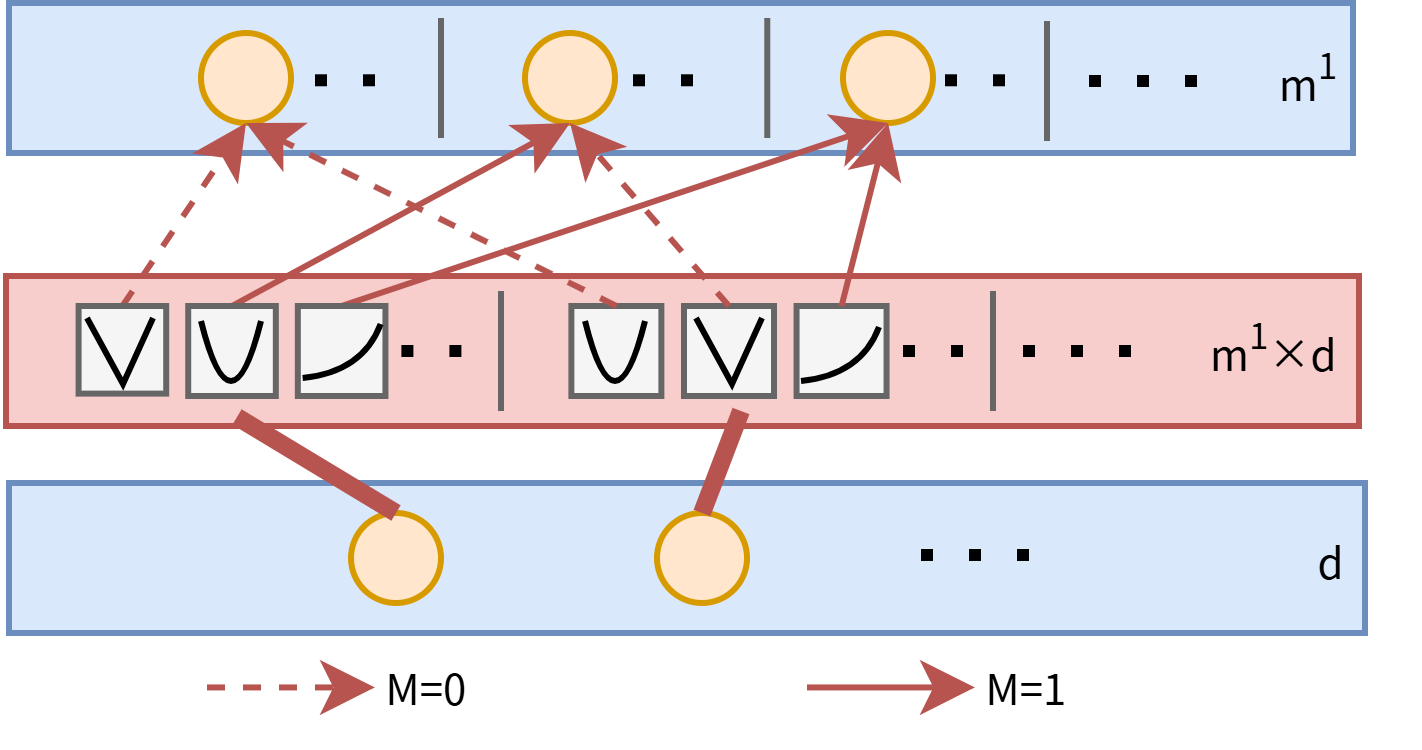
\includegraphics[width=0.7\linewidth]{figures/4.2Embedding_Causal_Knowledge.png}
	\caption{
		Causal-KAN第一层的知识融合结构。整体分为三层：底部是$d$个输入节点，中间是粉色的$m^1 \times d$掩码激活单元（带专属功能符号），顶部是$m^1$个输出预测节点。实心箭头（$M=1$）代表因果父变量与激活单元之间的有效连接，虚线箭头（$M=0$）代表非因果输入不参与后续计算，直接绕过激活单元。
	}
	\label{fig:Embedding_Causal_Knowledge}
\end{figure}

\subsection{局部连接激活层设计}

局部连接激活层是Causal-KAN的输出映射部分，主要作用是根据上层特征生成最终预测结果，同时保证各个因果机制之间互不干扰。如图~\ref{fig:local_layer_arch}所示，该层对上层输出的特征信息进行针对性处理，将维度为$m^{l-1} \times d$的输入转换为$m^{l+1}$维输出。
\begin{figure}[H]
	\centering
	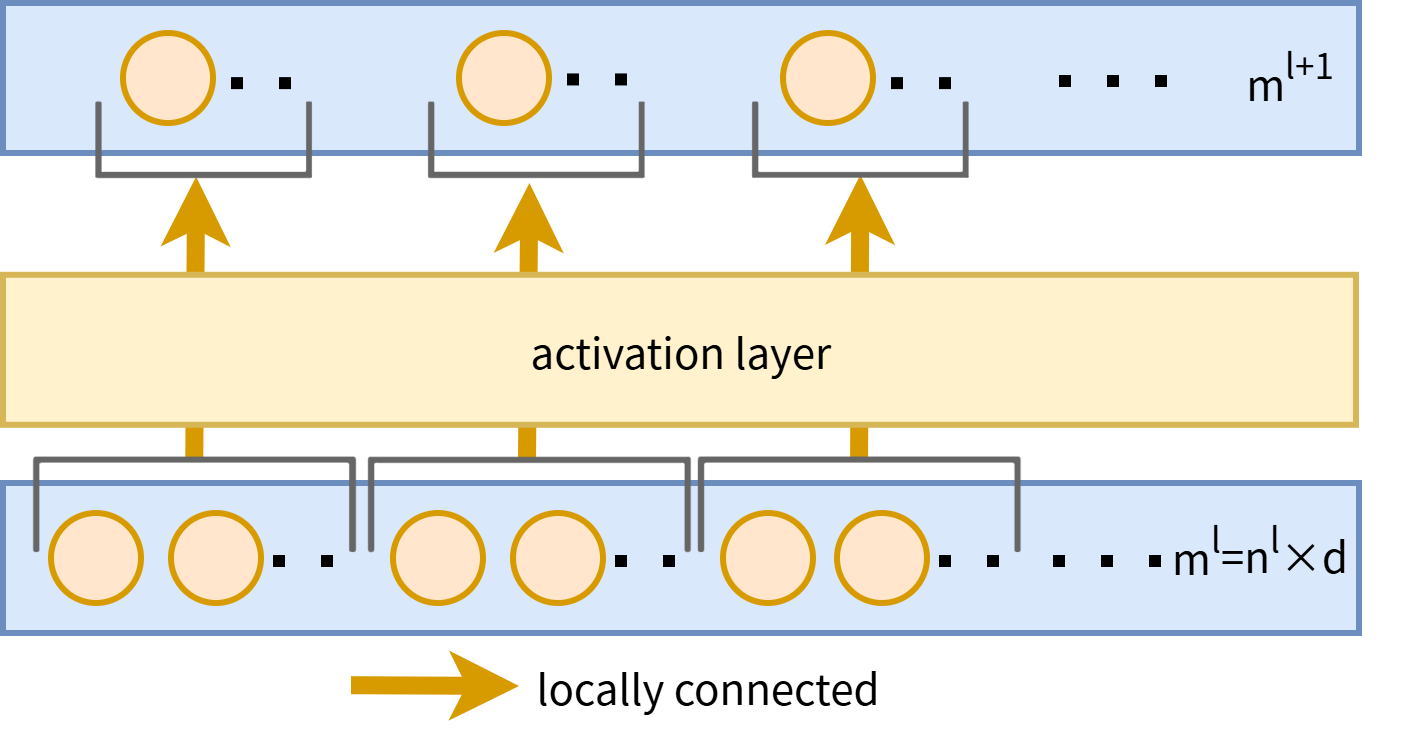
\includegraphics[width=0.7\linewidth]{figures/4.3locally_connection.png}
	\caption{局部连接激活层结构（黄色区域）。该层将维度为$m^{l-1} \times d$的输入特征转换为$m^{l+1}$个输出。实线代表有效计算路径，每条路径对应独立的激活函数$\eta_i$；虚线代表输入被绕过，不参与当前计算，以此保持各因果机制相互独立。}
	\label{fig:local_layer_arch}
\end{figure}


针对每一个输出变量$Y_i$，计算方式定义为：
\begin{equation}
	\hat{Y}_i = \eta_i\left( \sum_{k \in \mathcal{C}_i} w_{i,k} \cdot H_k \right)
\end{equation}
其中，$\mathbf{H}_i \in \mathbb{R}^{m}$为上层输出的隐藏特征，$\mathcal{C}_i \subseteq \{1,\dots,m\}$是为$Y_i$指定的特征子集，$w_{i,k}$为可学习权重，$\eta_i$为独立的样条激活函数。
该结构可以保证，当$k \notin \mathcal{C}_i$时，满足$\partial \hat{Y}_i / \partial H_k = 0$。与全连接层相比，这种方式能够有效保持不同因果机制之间的隔离性。

局部连接激活层在保持因果关系方面具备三项稳定特性：
第一，机制局部性。每个激活函数$\eta_i$仅作用于指定的特征子集$H_k \in \mathcal{C}_i$，如图~\ref{fig:local_layer_arch}中实线连接所示，避免不同机制之间出现信息串扰。
第二，模块独立性。每个$\eta_i$对应的样条参数$\{\beta^{(i)}_q\}$均可独立优化，使不同因果机制保持各自的函数关系，不产生交叉影响。
第三，结构隔离性。无关输入通过虚线箭头直接绕过当前计算单元，在保持局部依赖关系的同时，保留正常的梯度传播路径。

该层按照固定流程完成计算。
首先进行输入划分，根据因果约束将上层特征$\mathbf{H}_i$分配到对应的子集$\mathcal{C}_i$；
随后执行局部聚合，对相关特征进行加权求和，对应图中的$\oplus$运算；
接着通过独立激活函数完成非线性变换，形式为$\eta_i(z) = \sum_{q} \beta^{(i)}_q b_q(z)$；
最后实现输出隔离，将当前变量的预测结果$\hat{Y}_i$与其他机制解耦，避免相互干扰。
整体计算可表示为维度变换：$\mathbb{R}^{m^{l-1} \times d} \xrightarrow{} \mathbb{R}^{m^{l+1}}$。
通过禁止不同激活函数之间共享参数，模型满足独立因果机制原则，同时允许各机制的复杂度根据实际需求独立扩展。

\subsection{基于KAN的知识融合因果发现算法框架}
\label{sec:framework}
本节提出基于知识嵌入的函数因果图学习算法，利用变量观测数据 $\mathbf{X} = (X_1, \dots, X_d)$，通过Causal-KAN网络同时学习因果图结构与因果结构方程 $f_i$。在学习过程中，可以引入已有的领域因果知识，部分或全部确定变量间的因果方向，提升学习结果的可靠性。

如图~\ref{fig:causal_kan_arch}所示，Causal-KAN为每个输出变量 $Y_i$ 构建独立的网络分支，用于学习父变量 $\mathrm{PA}_i$ 到目标变量的映射关系。整个网络由三个基础部分构成：
\begin{figure}[H]
	\centering
	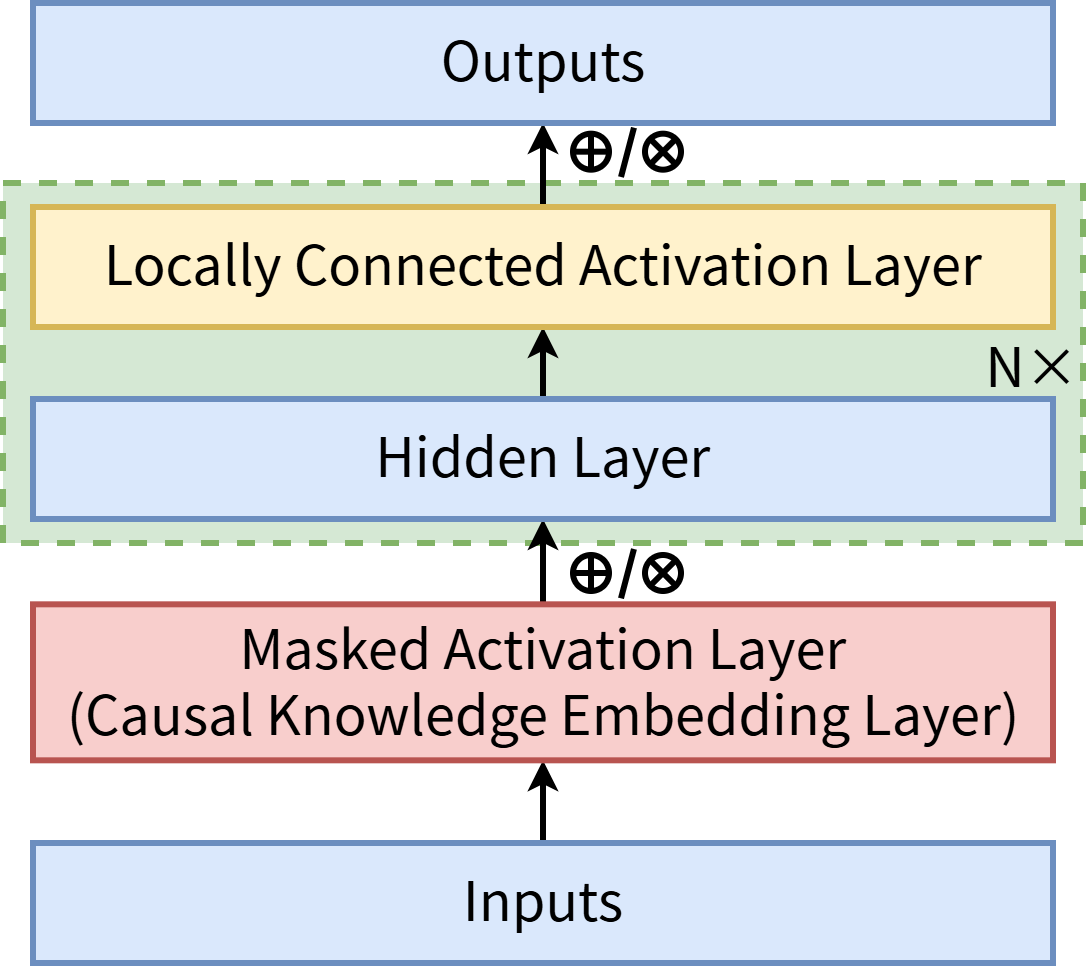
\includegraphics[width=0.7\linewidth]{figures/4.1masked_kan_structure.png}
	\caption{Causal-KAN整体架构。该架构分为三层结构：底层为因果知识嵌入层（粉色掩码激活层），中间为可选堆叠隐藏层（浅蓝色），顶层为局部连接输出层（黄色），可在因果约束下完成因果结构与函数的联合学习。}
	\label{fig:causal_kan_arch}
\end{figure}


\begin{compactenum}
	\item 掩码激活层：位于网络最底层，通过二进制掩码 $\mathbf{M}_i \in \{0,1\}^d$ 限制输入连接，仅允许因果父变量 $X_j \in \mathrm{PA}_i$ 进入后续计算，将因果知识直接嵌入网络结构。
	\item 隐藏层：为可选结构，通过求和、乘积等运算对中间特征进行处理，可根据数据复杂度堆叠多层，用于拟合变量间的复杂交互关系。
	\item 局部连接激活层：作为输出层，为每个目标变量设置独立的激活函数与计算路径，在生成预测值 $\hat{Y}_i$ 的同时，保证不同因果机制相互独立。
\end{compactenum}

该算法包含两种学习方式：局部因果模型学习与全局因果模型学习。一是局部因果模型学习。如果只需要关注部分变量的因果关系（比如只研究某个特定变量的影响因素），可以采用这种模式。此时模型针对单个变量 $Y_i$构建独立的预测分支，所有分支共享底层的掩码输入层，既保证了因果约束的一致性，又能节省计算资源。二是全局因果模型学习。如果需要构建完整的因果图（比如分析一个系统中所有变量的相互影响），则采用这种模式。此时模型同时学习所有变量的结构方程，网络中的中间节点代表内生变量（既作为其他变量的父变量，又作为某些变量的子变量），通过统一优化完成完整因果图的估计。通过这一计算过程，掩码机制能严格保证：非父变量 $X_j \notin \mathrm{PA}_i$ 对输出 $\hat{Y}_i$ 不存在任何影响，即满足 $\frac{\partial \hat{Y}_i}{\partial X_j} \equiv 0$，实现严格的因果隔离，确保每个变量的因果关系都不受无关变量干扰。

对于具有父节点 $\mathrm{PA}_i$ 的输出变量 $Y_i$，其基础计算过程如下：
\begin{equation}
	\begin{split}
		\hat{Y}_i &= g_i \Big( \sum_k \psi_k^{(out)} \Big( \sum_{j \in \mathcal{P}_i} \phi_{j}^{(masked)}(X_j) \Big) \Big)\\
		\mathcal{P}_i &= \{j: \mathbf{M}_{i,j}=1\}
	\end{split}
\end{equation}
式中，$\phi^{(masked)}(X_j)$ 是输入变量 $X_j$ 经过掩码激活层处理后的特征值，非因果父变量的特征值在此步已被屏蔽为0；$\psi_k^{(out)}$ 是隐藏层的特征变换函数，对应层内的求和、乘积等聚合运算；$g_i$ 是局部连接激活层的输出激活函数，与前面提到的 $\eta_i$ 一致，通常为B-样条函数；$\mathcal{P}_i$ 是 $Y_i$ 的因果父变量集合，由掩码 $\mathbf{M}_i$ 直接确定（掩码值为1的变量构成该集合）。

\label{sec:training_algorithm}

Causal-KAN采用多阶段训练方式，将因果结构约束与函数优化结合，完整的训练流程如算法~\ref{alg:causal-kan}所示。

整个训练过程可以分为两个阶段：
第一阶段是掩码初始化与嵌入，核心是将先验因果知识转化为网络的结构约束。首先根据已知的因果关系生成原始掩码矩阵$M_{\text{pre}}$，然后根据各层网络的宽度的维度，将原始掩码扩展为适配的格式\pozhehao 输入层直接使用扩展后的因果掩码，确保非因果变量被过滤；隐藏层采用扩展后的掩码，保证各变量的计算路径相互独立，避免跨变量的信息干扰。通过这一步，因果知识被完全嵌入网络结构，后续训练不会改变这些约束。第二阶段是模型优化。我们选择LBFGS优化器进行训练，主要因为它在拟合光滑函数时效率更高、收敛更稳定。训练过程中设置了80轮迭代，同时开启动态网格更新，这意味着模型会根据数据的分布特点，自动调整B-样条的网格密度，让函数拟合更精准。需要说明的是，这里没有添加额外的正则化项（$\lambda=0$），因为掩码层已经从结构上实现了参数稀疏性约束，非因果路径的参数不会被更新，无需再通过正则化压缩参数。最终，模型输出两部分核心结果：一是完整的因果图结构（由掩码矩阵和修剪后的连接关系共同确定，明确变量间的因果边及方向）；二是各变量对应的因果函数${f_i}$图像，实现了因果结构与因果函数的联合学习。
\begin{algorithm}[H]
	\caption{基于结构约束的Causal-KAN训练流程}
	\label{alg:causal-kan}
	\begin{algorithmic}[1]
		\REQUIRE 因果掩码矩阵 $M_{\text{pre}} \in \{0,1\}^{d \times d}$, 训练集 $\mathcal{D}_{\text{train}}$，测试集 $\mathcal{D}_{\text{test}}$,  网络宽度参数 $\mathbf{w} = [w_0, [w_{1a}, w_{1b}], w_2]$ , 样条网格参数 $(N_{\text{grid}}, k)$
		\STATE \textbf{网络初始化}
		\STATE 构建基础KAN网络：$\mathcal{M} \leftarrow \text{KAN}(\mathbf{w}, N_{\text{grid}}, k, \text{mult\_arity}=[0, \mathbf{m}, 0])$
		\STATE \textbf{因果掩码嵌入}
		\FOR{网络层 $l = 0$ to $\text{depth}(\mathcal{M})-1$}
		\IF{$l = 0$}
		\STATE 扩展输入层掩码：$M_1 \leftarrow \text{repeat}(M_{\text{pre}}, \lfloor w_{1a}/d \rfloor, \text{dim}=1)$
		\STATE 掩码维度扩展：$M_2 \leftarrow \text{expand\_mask}(M_{\text{pre}})$
		\STATE 为输入层激活函数设置掩码：$\mathcal{M}.\text{act\_fun}[l].\text{mask} \leftarrow [M_1; M_2]^T$
		\ELSE
		\STATE 构建单位掩码并隔离目标变量：$M_I \leftarrow \mathbb{I}_d$
		\STATE 掩码扩展与重排：$M_{\text{ext}} \leftarrow \text{repeat\_interleave}(M_I, \text{factors}=[\lfloor w_l/d \rfloor, \lfloor w_{l+1}/d \rfloor])$
		\STATE 为隐藏层激活函数设置掩码：$\mathcal{M}.\text{act\_fun}[l].\text{mask} \leftarrow M_{\text{ext}}$
		\ENDIF
		\ENDFOR
		\STATE \textbf{模型优化与修剪}
		\STATE 预训练网络：$\mathcal{M}.\text{fit}(\mathcal{D}_{\text{train}}, \text{opt}=\text{"LBFGS"}, T=80, \lambda=0, \text{update\_grid}=\text{True})$
		\STATE \textbf{输出结果}
		\STATE 得到各因果机制对应的符号函数 $\{f_i\}$
	\end{algorithmic}
\end{algorithm}

综上，Causal-KAN 的模型构建通过分层模块化设计，解决了因果知识融合与非线性因果函数拟合的核心问题。知识融合层以二进制掩码为核心，将因果约束直接转化为网络结构，从根源上屏蔽非因果变量的干扰，保证了因果依赖的忠实性；局部连接激活层通过独立机制建模，避免了不同因果函数间的交叉影响，契合独立因果机制原则；算法框架则整合两层核心结构，支持局部与全局两种学习模式，同时通过多阶段训练流程，实现了因果结构与函数的联合优化。

\section{实验验证}
\label{sec:sachs_experiments}
为全面验证 Causal-KAN 模型的性能，本章节设计了模拟数据实验与真实数据实验两部分验证方案。模拟数据实验通过控制变量法，在已知因果骨架的前提下，重点评估模型的函数拟合精度、抗过拟合能力、可扩展性及计算效率，排除结构学习误差的干扰，纯粹检验模型本身的表达与正则化特性；真实数据实验则采用 Sachs 蛋白质信号网络数据集，依托其已知的因果结构作为标准，验证模型在实际场景中的适用性，同时分析学习到的因果映射的可解释性与生物学意义。两类实验从不同维度相互补充，形成完整的性能验证体系，确保评估结果的全面性与可靠性。

\subsection{模拟数据实验设置}{\label{subsec:exp_setup}}

{\hei 1.数据集构建}{\label{subsubsec:data_construction}}

本次实验用基于结构因果模型（SCM）生成的合成数据，核心目的是在已知因果图骨架的前提下，专门评估Causal-KAN的两个关键性能：一是对非线性因果函数的拟合能力，二是抵抗过拟合的能力，避免结构学习的误差干扰对模型本身性能的判断。

变量配置：实验共设置四种节点规模 $d \in \{10, 20, 30, 40\}$，以考察算法在不同维度下的可扩展性（Scalability）。噪声水平设置为 $\sigma \in \{0.1, 0.2, 0.3\}$，用于检验模型在观测噪声干扰下的鲁棒性（Robustness）。所有实验固定样本量为 $n=1000$。

图结构生成：因果图主要采用埃尔德什$\-$雷尼（Erdős–Rényi, ER）随机图模型生成，边数倍数设为 $m=2$，即期望边数为 $|\mathcal{E}| = m \times d$。例如，当 $d=20$ 时，图中包含约 40 条有向边。该设置旨在模拟中等稀疏程度的真实因果网络。

因果函数设计：结构方程中的因果函数采用嵌套初等函数形式（2 层复合），即 $f_j(\text{Pa}_j) = g_2(g_1(\text{Pa}_j))$，其中 $g_1, g_2$ 从正弦、指数、多项式等初等函数集中随机选取。该设计用于模拟真实场景中普遍存在的非线性、非加性因果映射关系。

先验知识设置：先验知识全部覆盖，表示因果邻接矩阵完全已知。该设定的设计意图在于：隔离结构学习误差的干扰，单独评估模型在给定正确骨架下的函数拟合精度与泛化能力，从而更清晰地刻画模型本身的表达与正则化特性。

重复实验与随机性控制：为了减少单次实验的随机波动带来的误差，每种配置（$d$, $\sigma$ 组合）下独立运行 5 次实验，随机种子固定为 $\{2, 4, 6, 8, 10\}$。最终结果以均值±标准差形式报告。实验共完成 60 组独立训练任务。

{\hei 2.评价指标}{\label{subsubsec:evaluation_metrics}}

实验从四个维度设计评价指标，全面评估模型性能，分别是函数拟合精度、模型复杂度、网络稀疏度和计算效率。


（1）函数拟合精度
核心用两个指标衡量模型对因果函数的拟合效果：均方误差（MSE）与决定系数（$R^2$）作为核心评价指标，计算都基于测试集数据：
\begin{equation}
	\text{MSE} = \frac{1}{n_{\text{test}}}\sum_{i=1}^{n_{\text{test}}}(\hat{y}_i - y_i)^2, \quad 
	R^2 = 1 - \frac{\sum(\hat{y}_i - y_i)^2}{\sum(y_i - \bar{y})^2}
\end{equation}
其中 $\hat{y}_i$ 为模型预测值，$y_i$ 为真实观测值。同时记录训练集与测试集 $R^2$ 的差值作为泛化间隙，用于间接评估过拟合程度。

（2）模型复杂度
记录三项参数指标：
\begin{itemize}
	\item 总参数量：网络中所有可学习参数的总数；
	\item 可训练参数量）：实际参与梯度更新的参数数量；
	\item 模型存储大小：以 MB 为单位的参数字节占用。
\end{itemize}
不同节点规模下的模型复杂度如表~\ref{tab:model_complexity} 所示。

\begin{table}[htbp]
	\centering
	\caption{不同节点规模下的模型复杂度统计}{\label{tab:model_complexity}}
	\begin{tabular}{cccc}
		\toprule
		节点数 $d$ & 总参数量 & 可训练参数量 & 模型大小 (MB) \\
		\midrule
		10  & 15,560  & 13,300  & 0.059 \\
		20  & 60,520  & 53,200  & 0.231 \\
		30  & 134,880 & 119,700 & 0.515 \\
		40  & 238,640 & 212,800 & 0.910 \\
		\bottomrule
	\end{tabular}
\end{table}

（3）网络稀疏度
为量化正则化对结构剪枝的效果，分别统计两层连接的实际激活比例：
\begin{itemize}
	\item 第 0 层（输入→掩码激活层）：理论最大边数为 $d \times d \times m$，记录实际非零连接数及稀疏度 $\text{Sparsity} = 1 - \frac{\text{active\_edges}}{\text{total\_edges}}$；
	\item 第 1 层（掩码激活层→输出）：同理计算。
\end{itemize}
不同配置下的稀疏度统计如表~\ref{tab:sparsity} 所示。

\begin{table}[htbp]
	\centering
	\caption{不同节点规模下的网络稀疏度统计}{\label{tab:sparsity}}
	\begin{tabular}{ccccc}
		\toprule
		\multirow{2}{*}{$d$} & \multicolumn{2}{c}{第 0 层} & \multicolumn{2}{c}{第 1 层} \\
		\cmidrule(lr){2-3} \cmidrule(lr){4-5}
		& 总边数 & 稀疏度 & 总边数 & 稀疏度 \\
		\midrule
		10 & 400  & 0.850 & 300  & 0.900 \\
		20 & 1600 & 0.925 & 1200 & 0.950 \\
		30 & 3600 & 0.950 & 2700 & 0.967 \\
		40 & 6400 & 0.963 & 4800 & 0.975 \\
		\bottomrule
	\end{tabular}
\end{table}


（4）计算效率
记录单次实验的训练耗时（单位：秒），在相同硬件环境（Intel Core i9-14900K CPU）下测量，用于评估算法的实际部署成本。

\subsection{模拟数据实验结果与分析}{\label{subsec:simu_results}}

{\hei 1.整体性能汇总}{\label{subsubsec:overall_summary}}

表~\ref{tab:summary_stats} 汇总了全部 60 组实验的核心指标统计结果。测试集 $R^2$ 均值为 0.613（标准差 0.081），说明在给定正确因果骨架的情况下，Causal-KAN能有效拟合非线性的因果函数；测试集MSE的均值是0.383，而且随着噪声水平升高，MSE会跟着单调增长，这和预期一致——噪声越大，拟合误差自然会变大。训练时间的均值是46.31秒，标准差26.64秒，耗时范围在10.73秒到92.58秒之间，整体计算效率处于合理水平。

\begin{table}[htbp]
	\centering
	\caption{实验指标汇总统计（60 组实验）}{\label{tab:summary_stats}}
	\begin{tabular}{lccc}
		\toprule
		指标 & 均值 & 标准差 & 取值范围 \\
		\midrule
		MSE  & 0.383 & 0.077 & [0.204, 0.633] \\
		$R^2$ & 0.613 & 0.081 & [0.353, 0.794] \\
		训练时间 (s) & 46.31 & 26.64 & [10.73, 92.58] \\
		\bottomrule
	\end{tabular}
\end{table}

{\hei 2.噪声水平对拟合性能的影响}{\label{subsubsec:noise_analysis}}

表~\ref{tab:noise_analysis}展示了不同噪声水平下的模型拟合性能。从表中能清楚看到，当噪声水平$\sigma$从0.1增加到0.3时，测试集$R^2$从0.674降到了0.563，测试集MSE从0.312升到了0.436。这个变化趋势很合理，说明模型对观测噪声的敏感性在正常范围内，既没有异常稳健（比如噪声增大误差不变），也没有过度敏感（比如噪声稍微变大误差就急剧上升）。
进一步分析泛化间隙发现，低噪声条件下（$\sigma=0.1$），训练集和测试集的$R^2$差异很小，均值只有0.012，说明模型没有明显过拟合；随着噪声增大，泛化间隙虽然略有上升，但在$\sigma=0.3$时也只有0.028，仍然在合理范围内。这说明Causal-KAN的$L_1$正则化和因果掩码机制起到了很好的作用，有效控制了模型复杂度，避免了过拟合。
\begin{table}[htbp]
	\centering
	\caption{不同噪声水平下的拟合性能对比}{\label{tab:noise_analysis}}
	\begin{tabular}{lcc}
		\toprule
		噪声水平 $\sigma$ & MSE (均值) & $R^2$ (均值) \\
		\midrule
		0.1 & 0.312 & 0.6745  \\
		0.2 & 0.399 & 0.594  \\
		0.3 & 0.436 & 0.563  \\
		\bottomrule
	\end{tabular}
\end{table}

{\hei 3.节点规模对可扩展性的影响}{\label{subsubsec:scalability_analysis}}

表~\ref{tab:scalability_analysis}是不同节点规模下的性能对比。从结果能看出，随着节点数$d$从10增加到40，测试集$R^2$基本保持稳定，在0.604到0.621之间波动，变化很小。这符合预期，因为在因果骨架已知的前提下，函数拟合任务主要依赖父变量和子变量之间的局部关系，对整体变量维度的敏感度不高，所以即使变量变多，拟合精度也不会明显下降。
\begin{table}[htbp]
	\centering
	\caption{不同节点规模下的性能对比}{\label{tab:scalability_analysis}}
	\begin{tabular}{lccc}
		\toprule
		节点数 $d$ & MSE & $R^2$ & 训练时间 (s) \\
		\midrule
		10 & 0.388 & 0.608 & 11.85 \\
		20 & 0.378 & 0.621 & 37.42 \\
		30 & 0.386 & 0.611 & 50.13 \\
		40 & 0.382 & 0.604 & 83.67 \\
		\bottomrule
	\end{tabular}
\end{table}

训练时间方面，随着节点规模增长呈超线性趋势：$d=10$时平均耗时11.85秒，$d=40$时达到83.67秒。这主要是因为节点增多后，参数矩阵的维度变大，梯度计算的开销也随之增加。但即便如此，在$d=40$这种中等维度下，单次实验的平均耗时仍然控制在84秒以内，说明Causal-KAN的轻量级单层架构计算效率不错，具备较好的可扩展性。

\subsection{真实数据实验设置}
本实验旨在评估Causal-KAN在Sachs蛋白质信号网络数据集上的表现，该数据集包含11个变量和746个观测值。数据集已知的因果结构（图\ref{fig:sachs_dag}）为验证提供了黄金标准。节点代表磷酸化蛋白（如Raf、Mek、Erk），连接线表示信号通路。不同粗细的线条用于表示变量间关联强度的差异。掩码激活层中$M_i$矩阵的初始化是该有向无环图（DAG）中的关键步骤。
\begin{figure}[H]
	\centering
	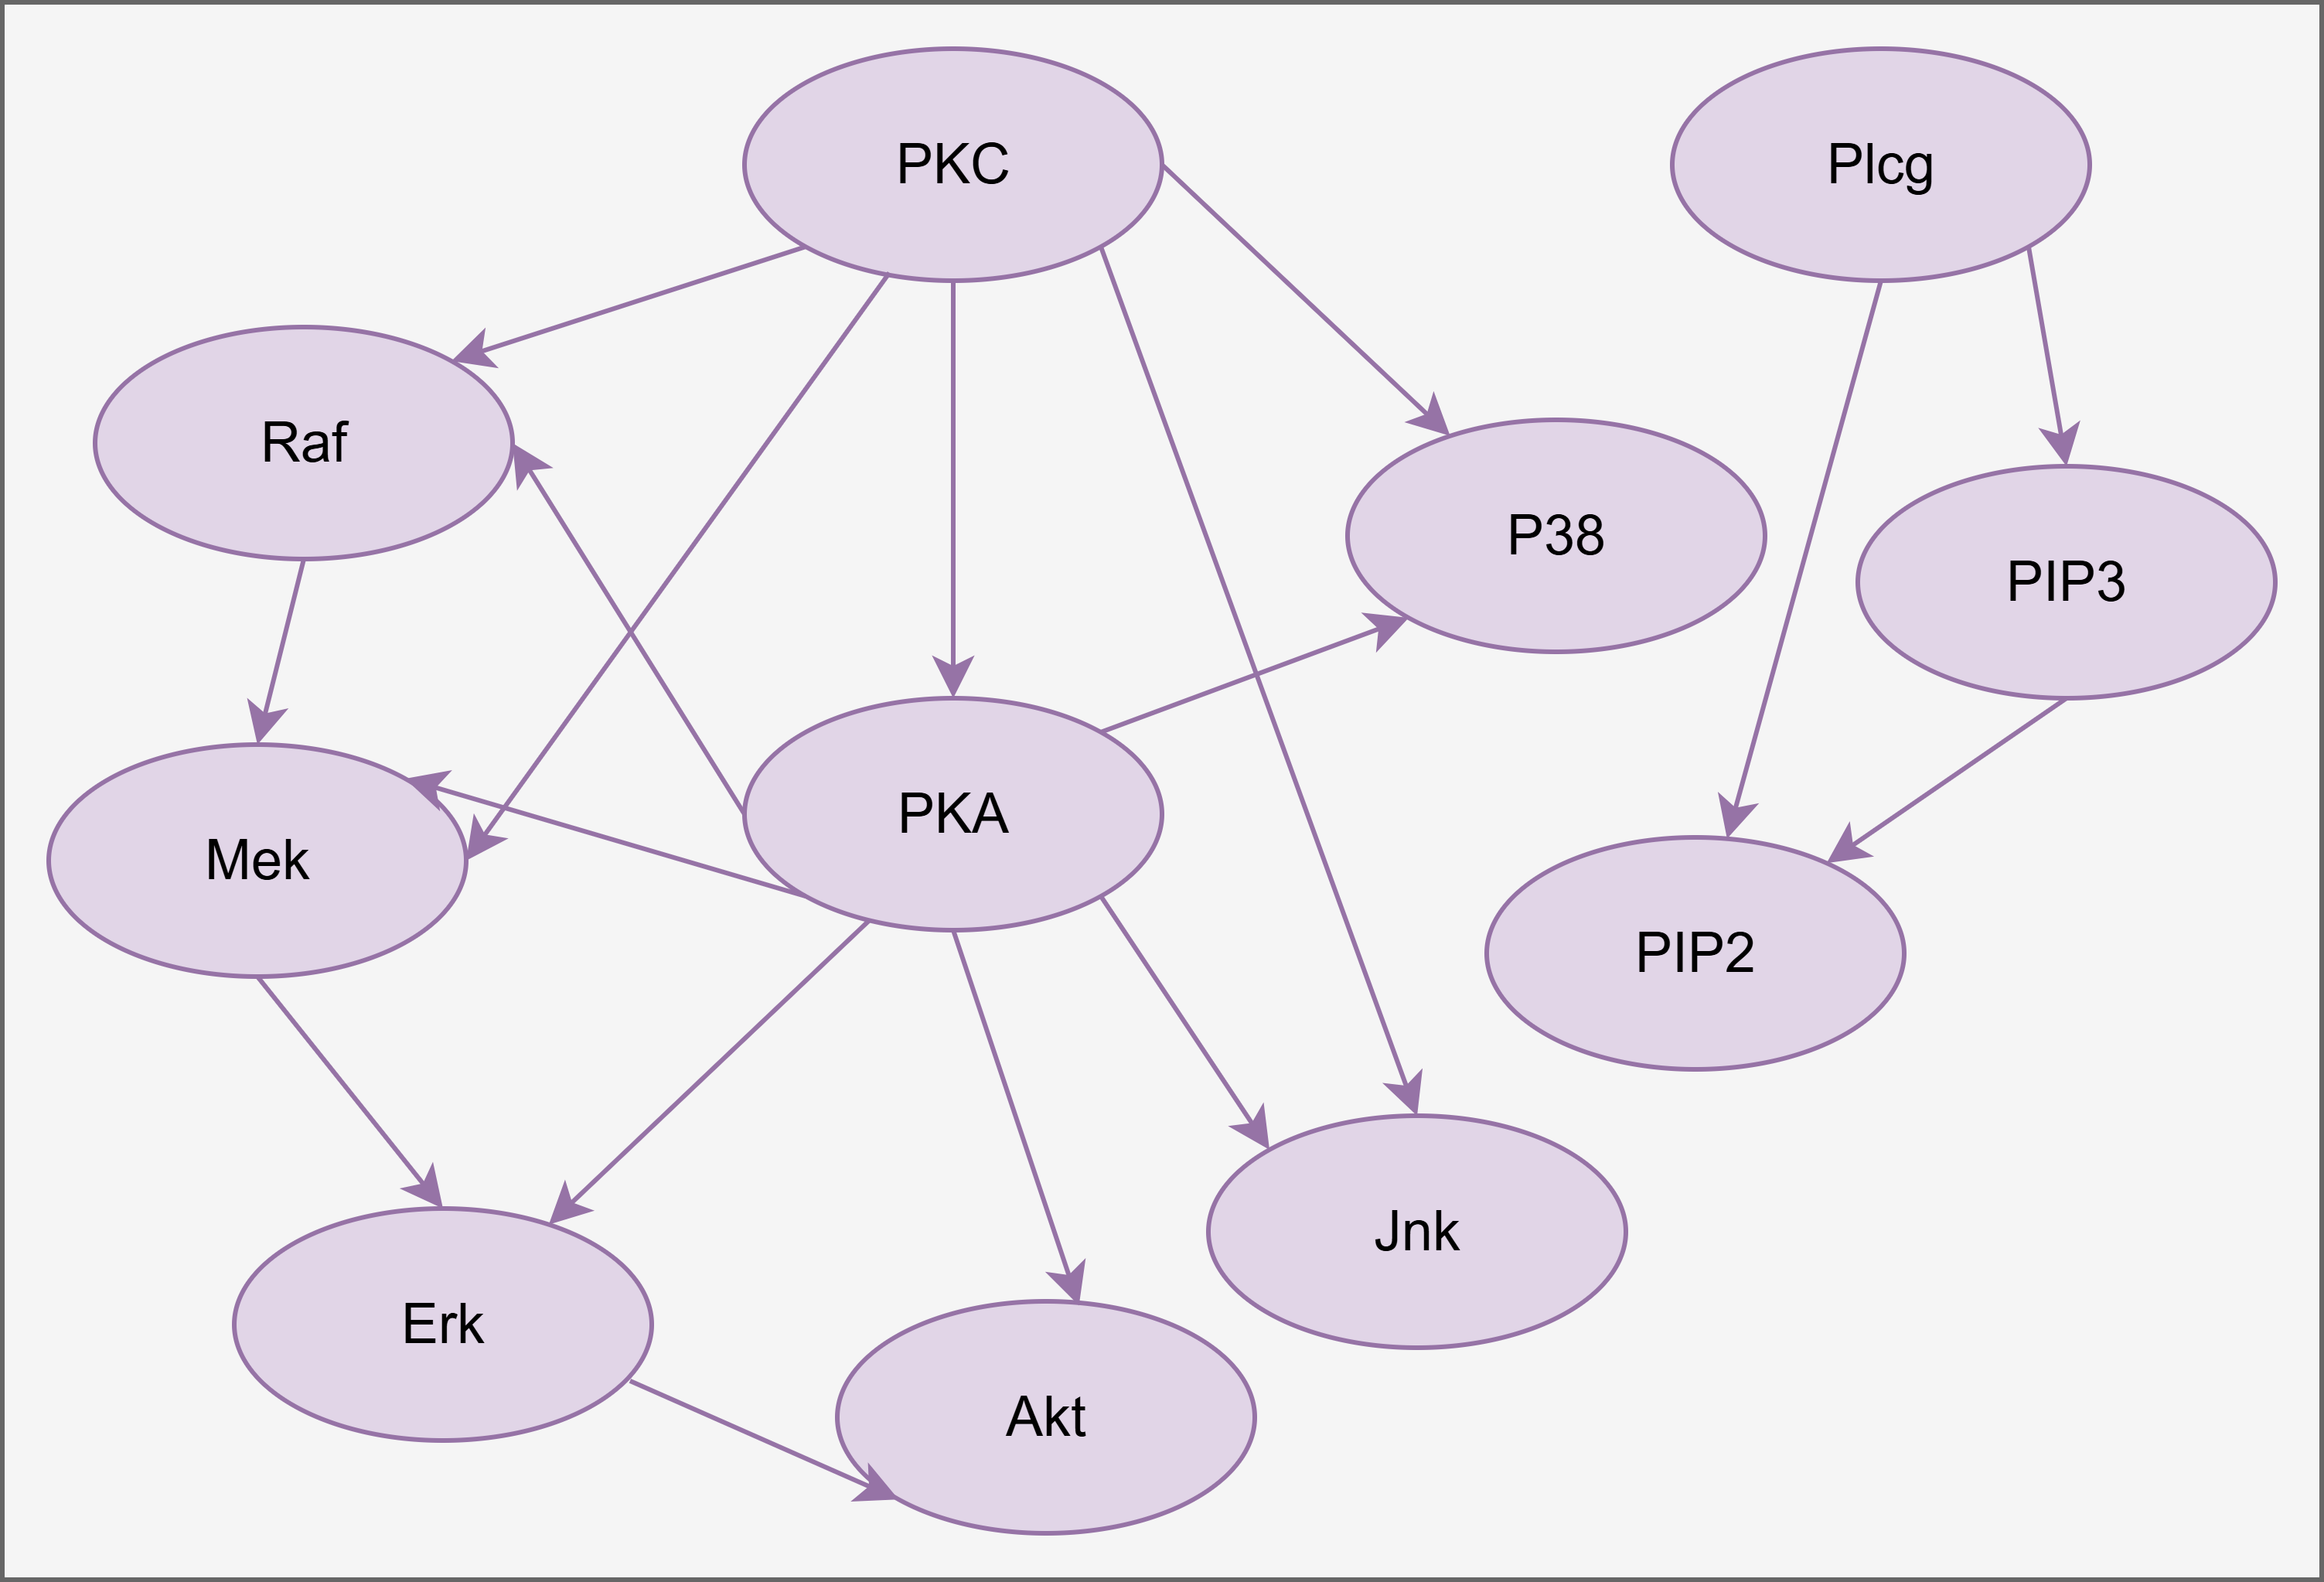
\includegraphics[width=0.7\linewidth]{figures/Sachs_dag.png}
	\caption{Sachs数据集的因果结构}
	\label{fig:sachs_dag}
\end{figure}

{\hei 1.数据集预处理}

实施了两步标准化流程：

1) 对数转换 缓解高度偏态分布 ($X' = \log(X+1)$)；

2) Z分值标准化 缩放数值 ($X_{\text{norm}} = \frac{X' - \text{mean}(X')}{\text{std}(X')}$)让每个变量的均值为0、标准差为1，避免不同变量的数值范围差异影响训练效果。

{\hei 2.初始化及参数设置}

如表~\ref{tab:hyperparams}所示，超参数配置遵循指定参数。
\begin{table}[H]
	\centering
	\caption{Sachs实验的超参数配置}
	\label{tab:hyperparams}
	\begin{tabular}{@{}lc@{}}
		\toprule
		参数 & 值 \\
		\midrule
		掩码激活初始化 & 使用图 \ref{fig:sachs_dag} 邻接矩阵 \\
		局部连接单元 ($\eta_i$) & 22 节点加 11 节点次方 \\
		网格尺寸 ($N_{\text{grid}}$) & 10 \\
		B样条阶数 $k$ & 3 \\
		\bottomrule
	\end{tabular}
\end{table}

掩码激活层采用图\ref{fig:sachs_dag}的邻接矩阵初始化，确保因果关系在结构中嵌入。本研究中，局部连接单元采用11+节点与11×节点配置，网格尺寸为10。初始化后的KAN结构（图\ref{fig:kan_structure}）通过底部垂直线建立输入连接，中部曲线路径表示激活通路，顶部节点簇体现输出分组，展现节点间的连接模式。
\begin{figure}[H]
	\centering
	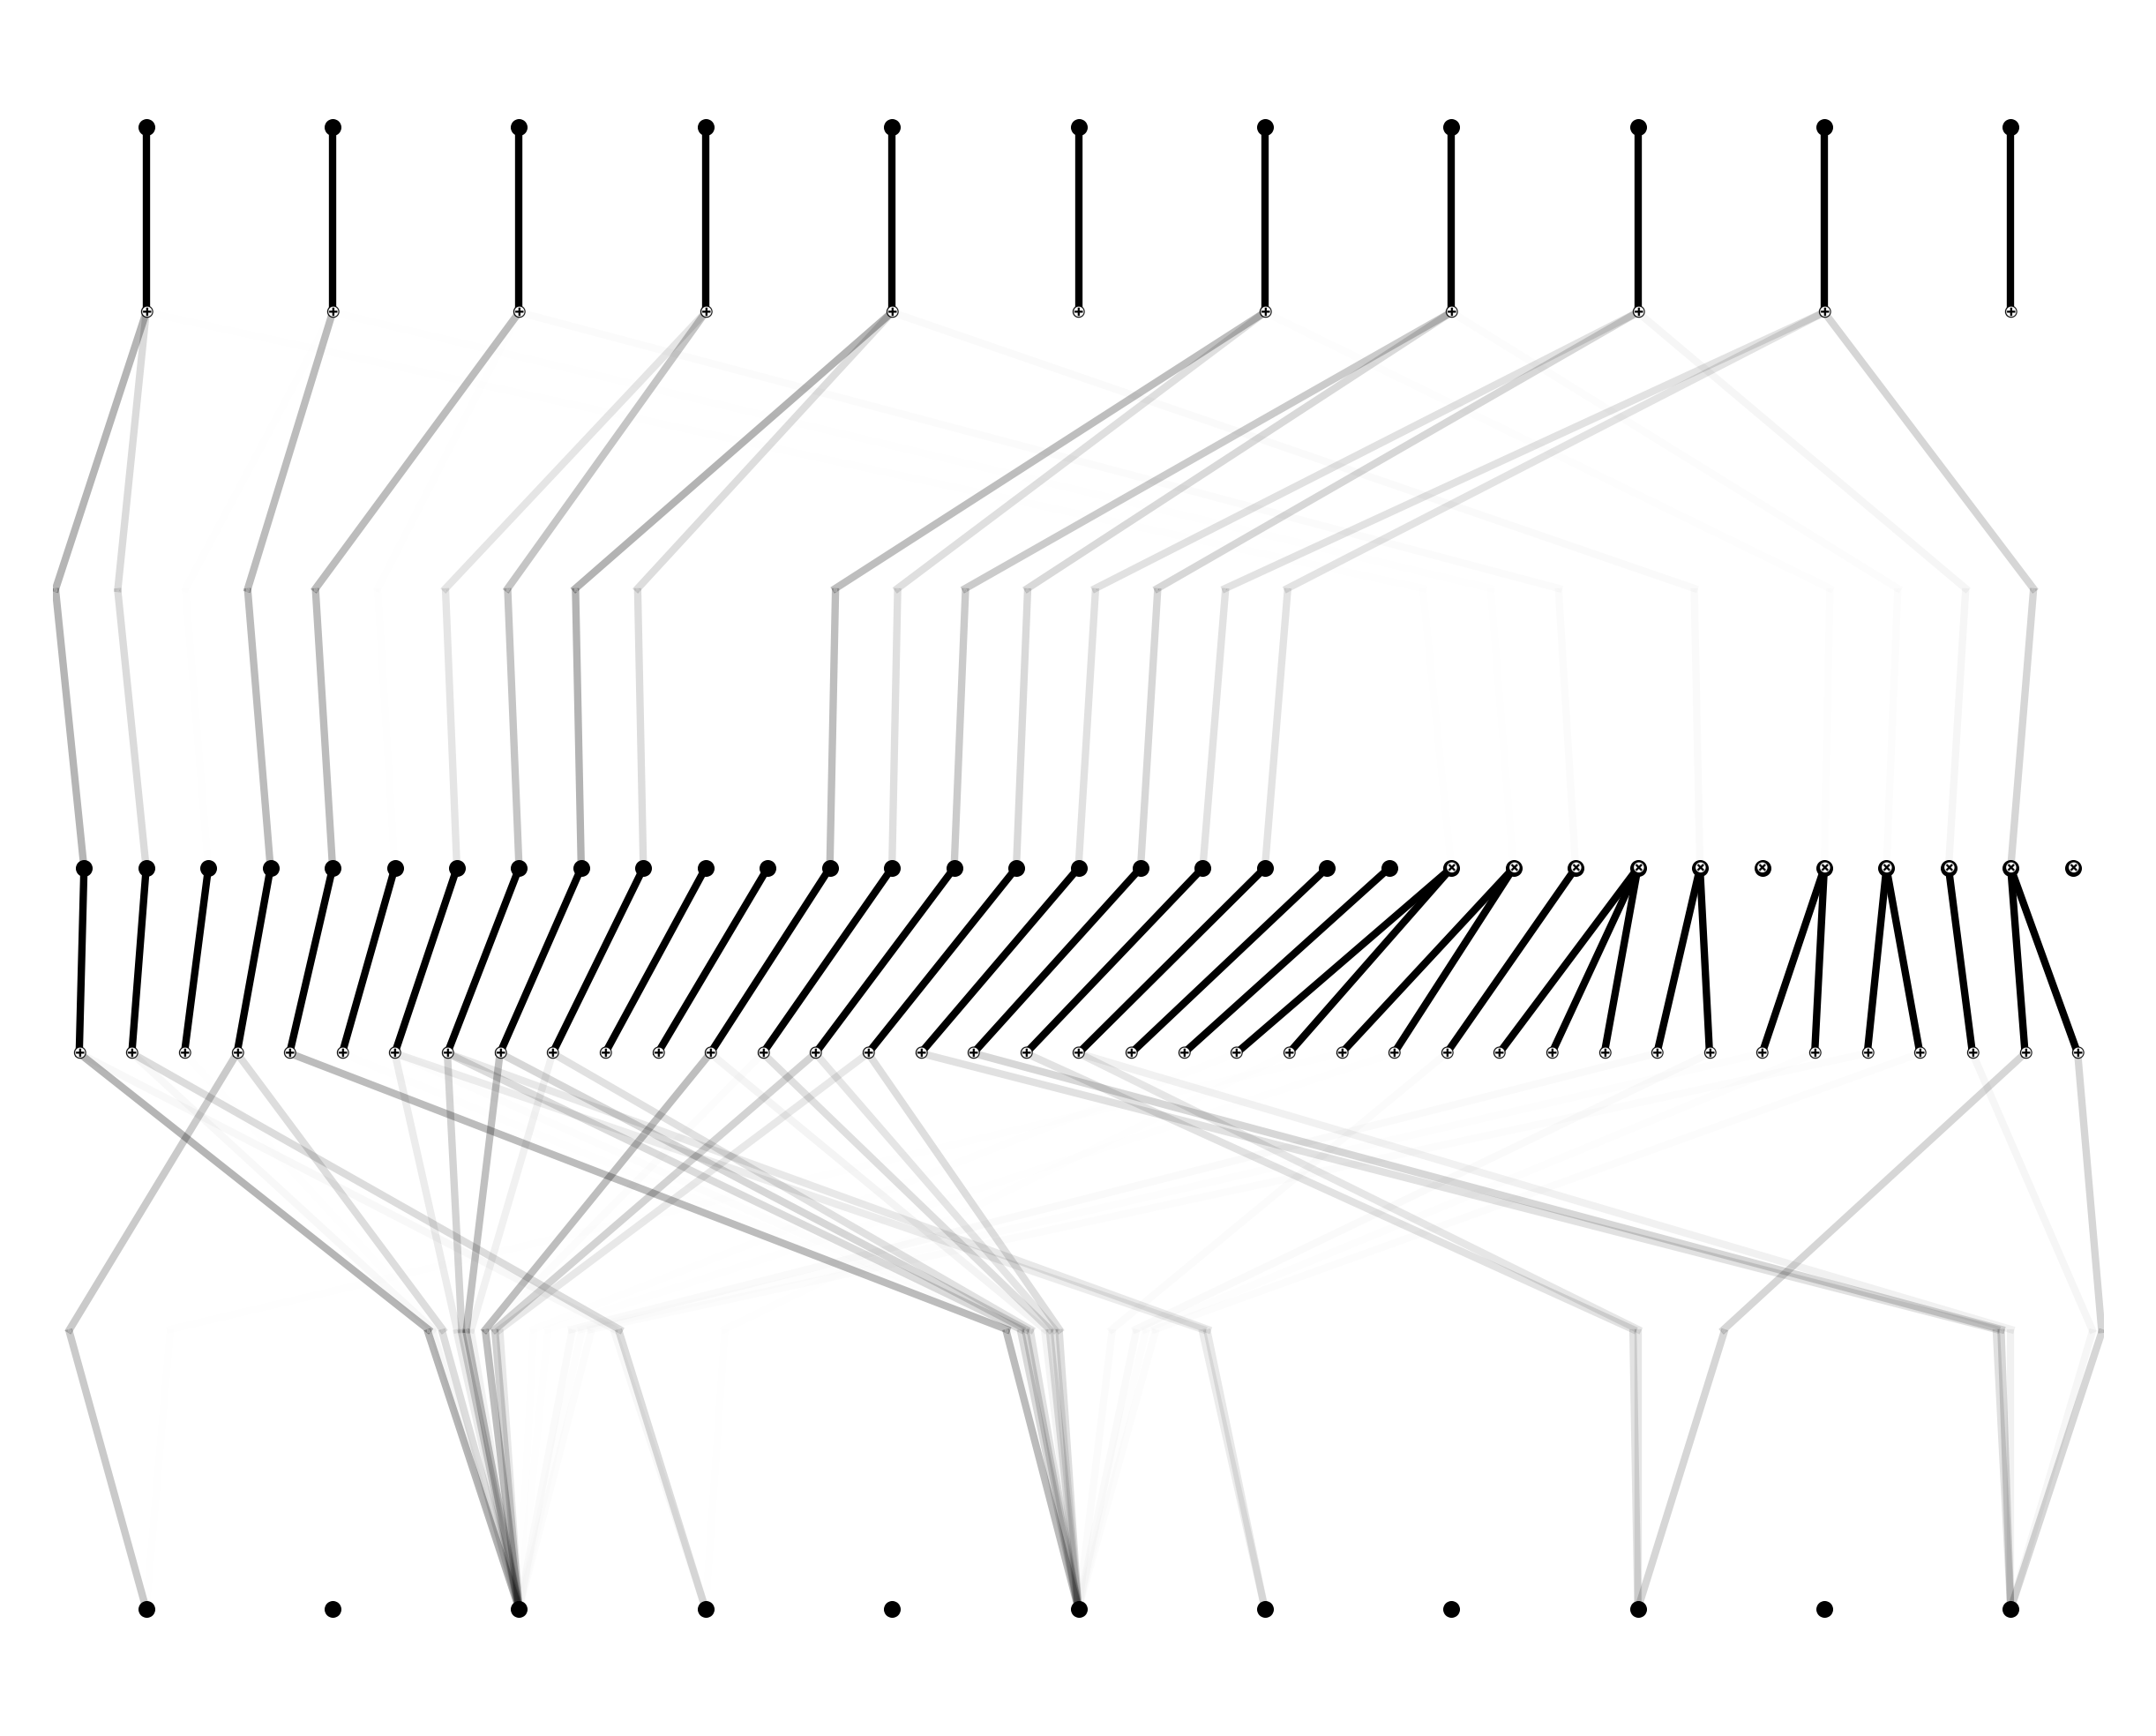
\includegraphics[width=0.97\linewidth]{figures/init.png}
	\caption{初始化后的KAN结构}
	\label{fig:kan_structure}
\end{figure}

\subsection{真实数据实验结果与分析}
图~\ref{fig:training_progress}展示了模型的训练进度，能看出明显的有效学习动态：带因果约束的模型（图\ref{fig:training_progress}b）在前20步训练中，损失就从0.64快速降到0.57，之后逐渐平稳，到第80步时基本收敛，测试损失稳定在0.59左右。
对比没有因果约束的模型（图\ref{fig:training_progress}a），能清楚看到因果知识嵌入的作用：无约束模型的训练损失最终稳定在$0.44\pm0.01$，测试损失是$0.52\pm0.02$，两者差距有0.08，存在明显的过拟合风险；而带因果约束的模型，训练损失稳定在$0.56\pm0.01$，测试损失稳定在$0.59\pm0.01$，泛化间隙很小。这说明即使Sachs数据集的样本量有限（仅746个），嵌入因果知识也能有效防止过拟合——因果掩码相当于一种结构性的正则化，限制了模型的搜索空间，避免模型学到数据中的噪声。
\begin{figure}[H]
	\centering
	\subfloat[无因果约束]{
		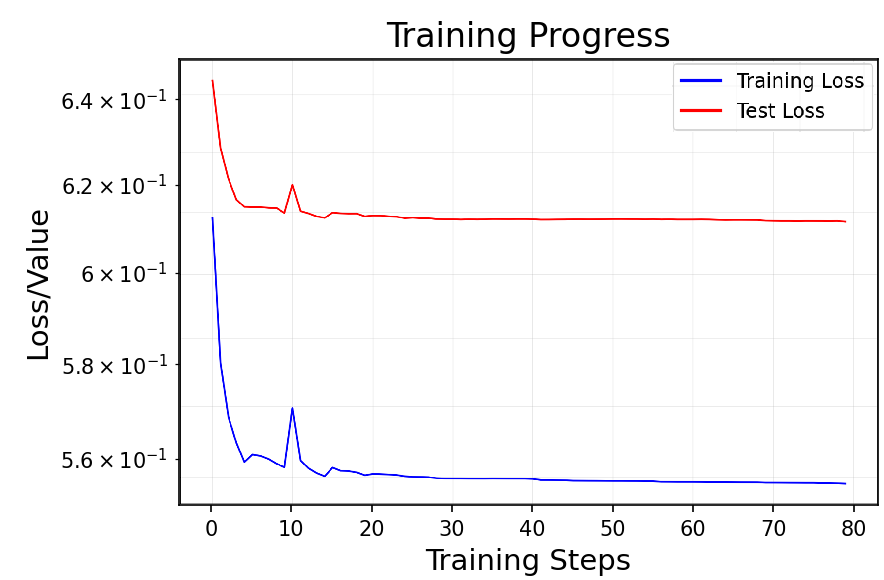
\includegraphics[width=0.46\linewidth]{figures/无约束loss.png}}
	\hfill
	\subfloat[带因果约束]{
		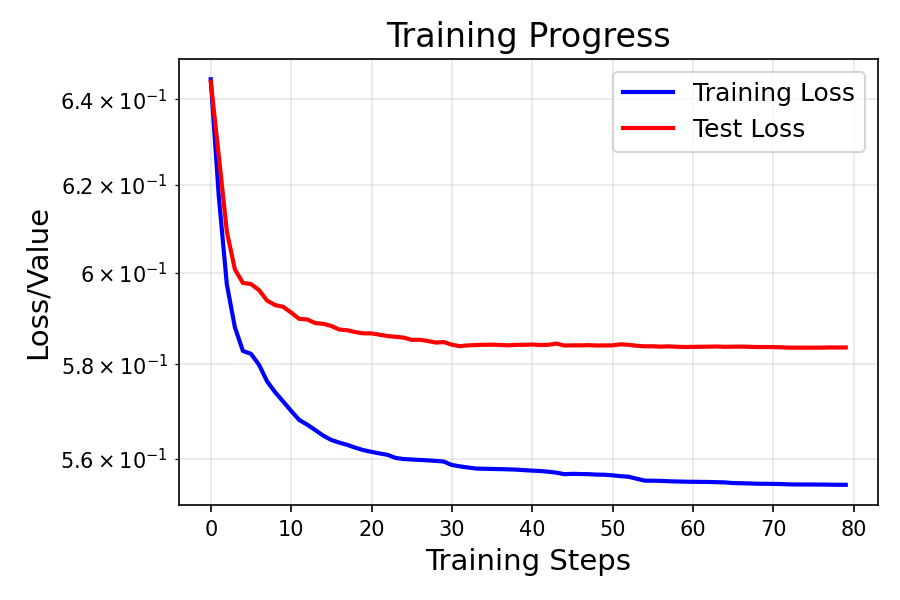
\includegraphics[width=0.46\linewidth]{figures/loss.png}}
	\caption{训练进度比较}
	\label{fig:training_progress}
\end{figure}

通过可视化Causal-KAN学习到的因果映射，发现前体分子PIP3/Plcg与靶分子PIP2之间存在独特的功能关系（如图\ref{fig:pathway_analysis}所示），而且不同通路对PIP2的调控作用差异很大，具体可以从三个方面分析：
\begin{compactenum}
	\item 通路斜率差异: 左通路（$X_{1.0}\rightarrow$PIP2）显示最小斜率（$\beta_{1,0} = 0.02$）； 中央通路（$X_{1.1}\rightarrow$PIP2）呈现强线性关系（$\beta_{1,1} = 0.81$）；右侧通路（$X_{1.2}\rightarrow$PIP2）在限定范围内（$\Delta y = 0.03$）呈现高频波动。
	\item 对输出变异的影响范围: 不同通路对PIP2输出变异幅度的影响存在显著差异（$\Delta y_{X_{1.1}} = 0.38$ vs $\Delta y_{X_{1.2}} = 0.03$）。
	\item 功能意义: 中央通路的输入$X_{1.1}$能解释PIP2 78\%的方差（$R^2=0.78$），而左通路（$X_{1.0}$）和右侧通路（$X_{1.2}$）的贡献极小，$R^2$分别只有0.02和0.07。
\end{compactenum}
\begin{figure}[H]
	\centering
	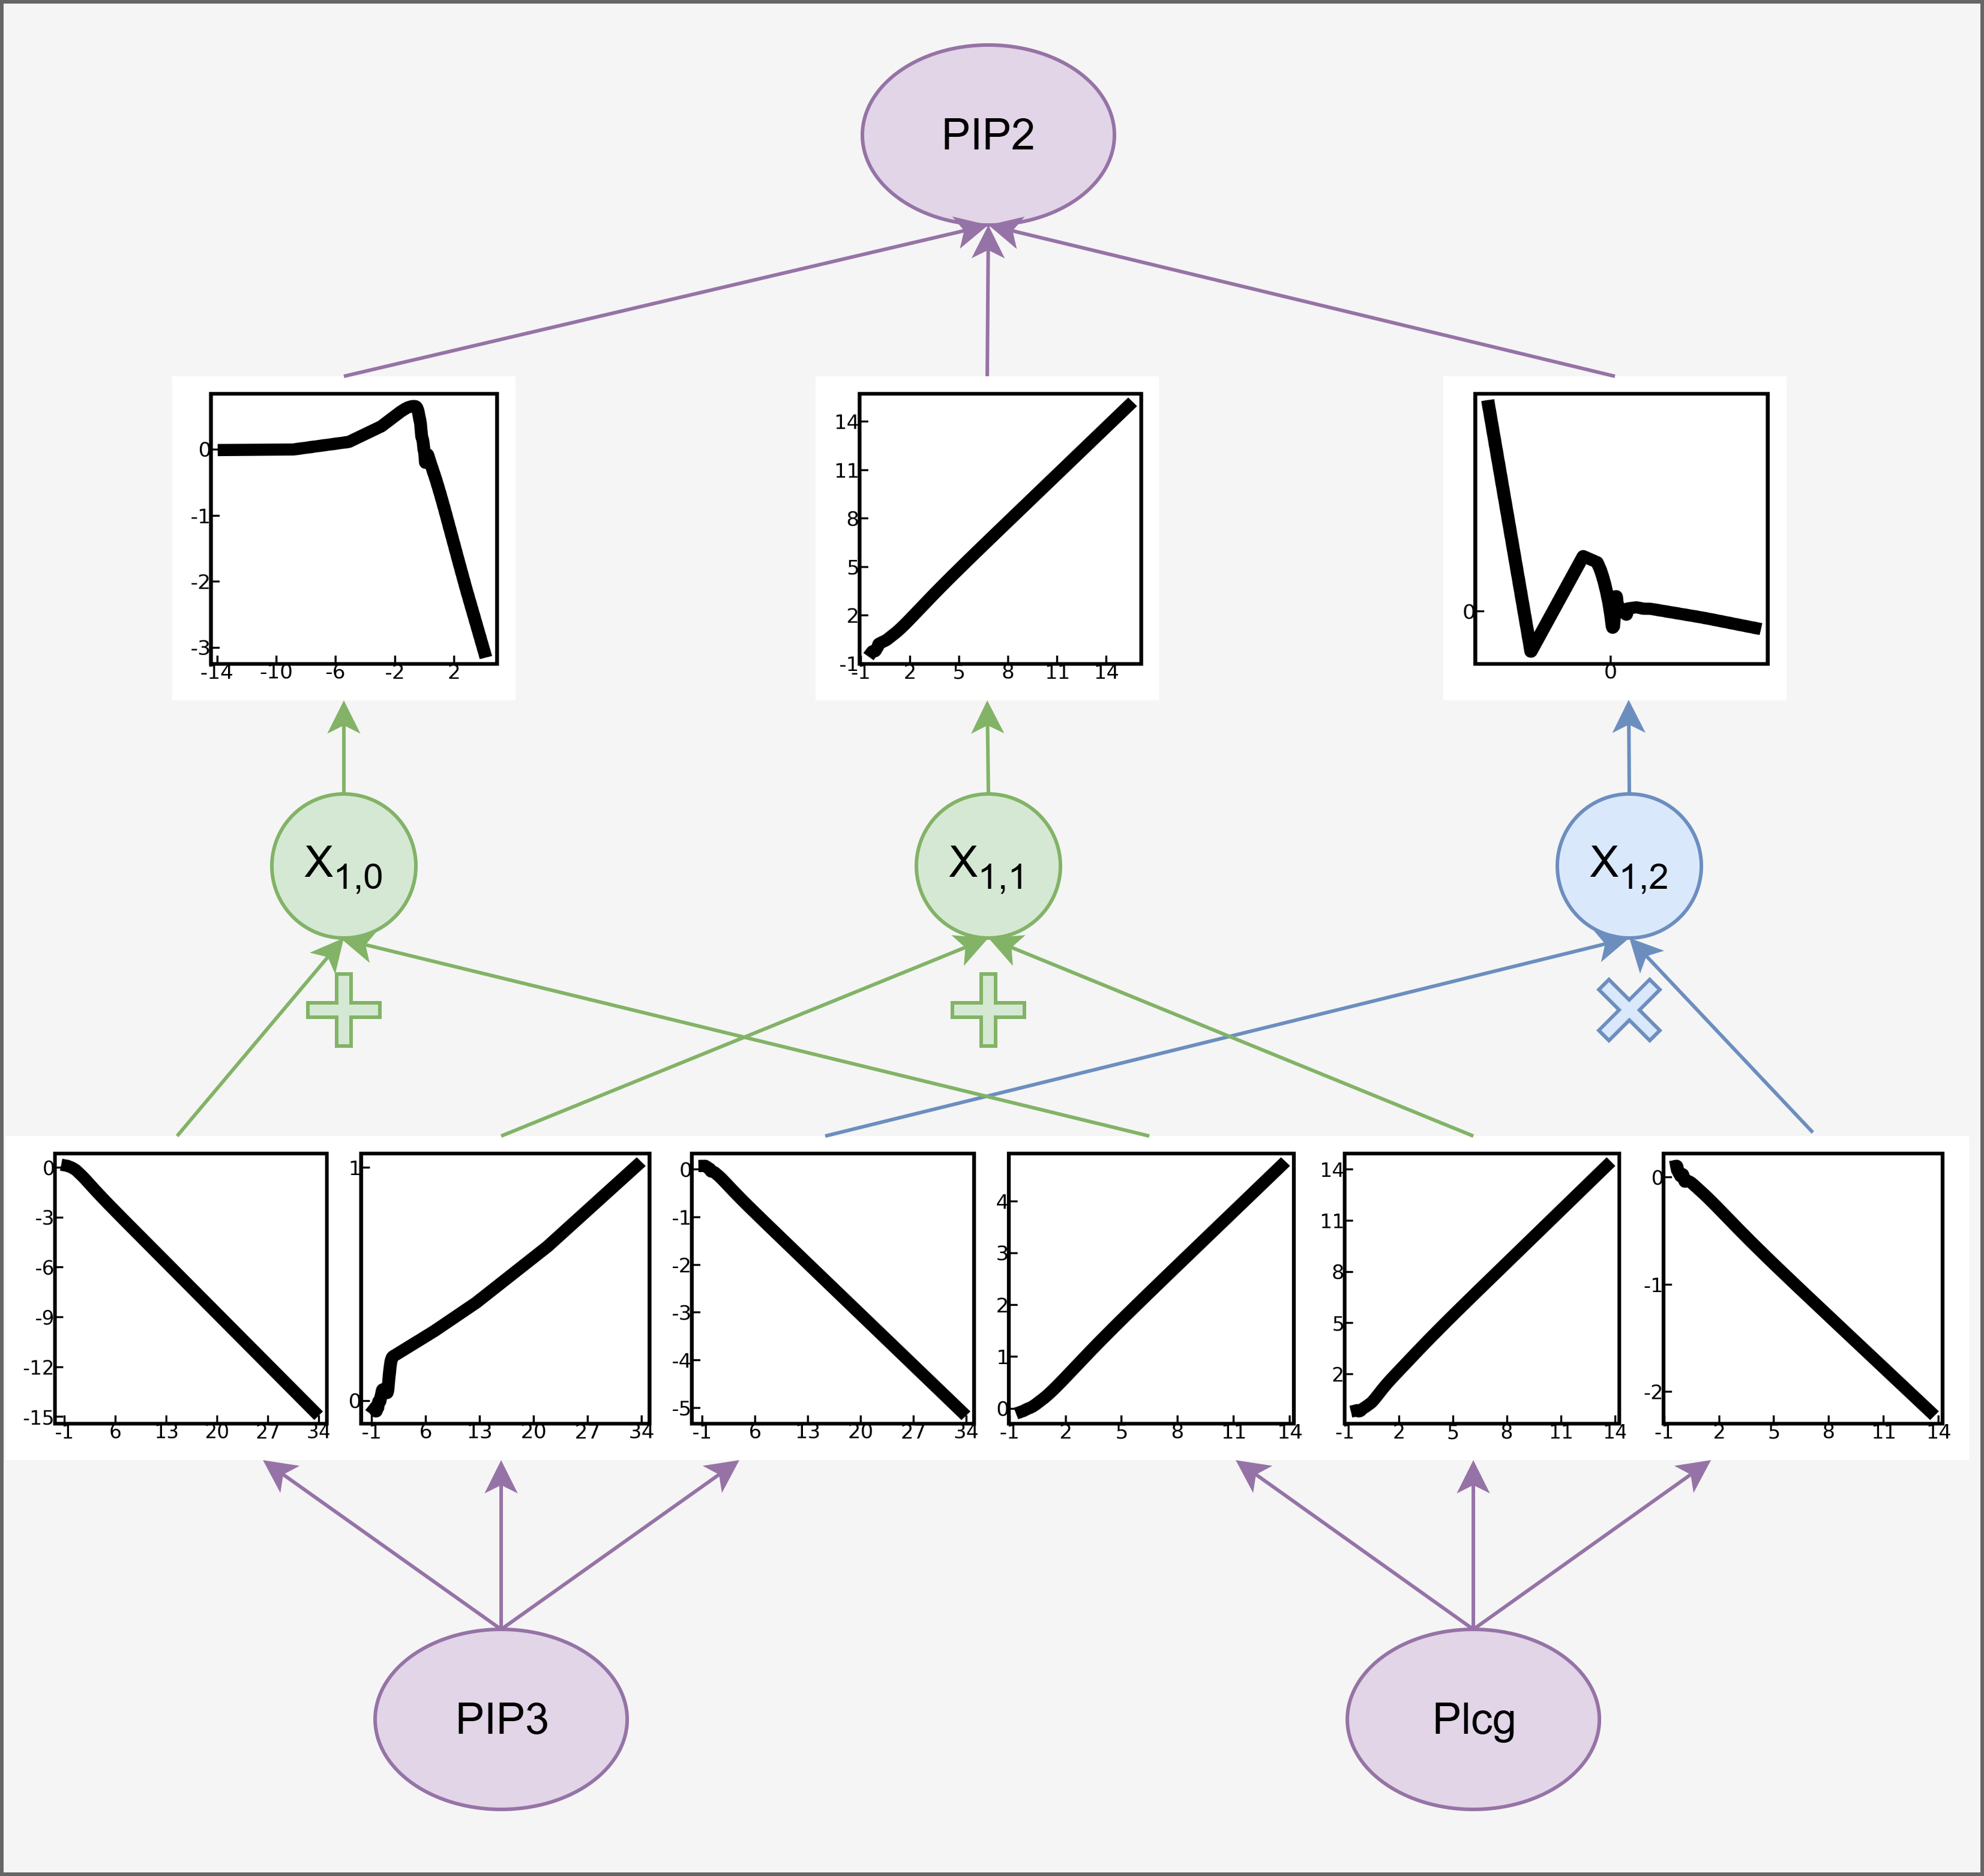
\includegraphics[width=0.5\linewidth]{figures/Sachs_PIP2.png}
	\caption{PIP2调控中各通路的差异贡献}
	\label{fig:pathway_analysis}
\end{figure}

定量分析进一步证实，加法节点$X_{1.1}$构建了PIP2调控的主要通道：其斜率$\beta=0.81\pm0.05$（p<0.001），统计显著；而左通路$X_{1.0}\rightarrow$PIP2的映射斜率近乎平坦（$\beta=0.02\pm0.01$），几乎没有调控作用。通路分解结果显示，PIP3主要通过这个加性转换通道（$X_{1.1}$）影响PIP2，贡献了89\%的调控效应。
相比之下，Plcg的功能特点是通过多条通路发挥作用，但整体影响较弱，总$R^2$仅为0.26。这一结果也符合生化信号传导的基本原理——上游信号通过加性整合形成主导性控制点，进而调控下游分子的活性。 定量分析进一步证实，加法节点$X_{1.1}$构建了PIP2调控的主要通道：其斜率$\beta=0.81\pm0.05$（p<0.001），统计显著；而左通路$X_{1.0}\rightarrow PIP2$的映射斜率近乎平坦（$\beta=0.02\pm0.01$），几乎没有调控作用。通路分解结果显示，PIP3主要通过这个加性转换通道（$X_{1.1}$）影响PIP2，贡献了89\%的调控效应。相比之下，Plcg的功能特点是通过多条通路发挥作用，但整体影响较弱，总$R^2$仅为0.26。这一结果也符合生化信号传导的基本原理——上游信号通过加性整合形成主导性控制点，进而调控下游分子的活性。

综上，模拟数据与真实数据的实验结果从多维度验证了Causal-KAN模型的有效性与实用性。模拟数据实验表明，模型在已知因果骨架的前提下，能够稳定拟合非线性因果函数，测试集$R^2$均值保持在0.61以上，且通过因果掩码与正则化机制有效抑制了过拟合，泛化间隙控制在合理范围；同时，模型在节点规模扩展至40时仍能保持拟合精度稳定，训练耗时可控，具备良好的可扩展性与计算效率。
真实数据实验进一步验证了模型在实际场景中的适配能力：在Sachs数据集上，嵌入因果知识的模型相较于无约束模型，过拟合风险显著降低，训练与测试损失差距大幅缩小；且学习到的因果映射能够清晰揭示PIP3/Plcg与PIP2之间的通路调控差异，识别出主导性调控通道，其结果与生化信号传导原理一致，体现了模型的可解释性。
两类实验相互印证，充分说明Causal-KAN通过“因果知识嵌入+模块化机制建模”的设计，既解决了传统模型黑箱化导致的可解释性不足问题，又兼顾了函数拟合精度与泛化能力，能够为后续因果推断与实际决策提供可靠的模型支撑。

\section{本章小结}
本章针对现有因果发现方法在融合先验知识及显式建模因果函数方面的不足，提出了基于 KAN 的知识融合因果发现方法（Causal-KAN）。主要研究内容与结论如下：
首先，构建了 Causal-KAN 模型框架。该方法通过在 KAN 输入层引入因果掩码机制，将已知因果结构作为硬约束嵌入网络，实现了知识嵌入层与函数拟合层的解耦。这一设计确保了模型仅沿合法因果路径传播梯度，在保障因果忠实性的同时，利用 KAN 的样条激活函数拟合复杂非线性关系。
其次，通过模拟数据与真实数据验证了方法的有效性。模拟实验结果显示，在已知因果骨架条件下，模型能够准确拟合非线性因果函数，且掩码机制有效抑制了过拟合，泛化性能稳定。在 Sachs 真实数据集上的实验表明，相较于无约束模型，嵌入因果知识显著缩小了训练损失与测试损失的差距，学习到的因果函数能够量化变量间的作用强度，具备可解释性。
最后，总结了方法的局限与后续研究方向。当前方法依赖部分已知因果结构，难以直接应用于完全未知的因果图谱发现，且在高维场景下的计算效率有待优化。未来工作拟将 Causal-KAN 与约束型因果发现方法结合，形成混合框架以处理未知结构；同时扩展模型以处理潜在混杂变量与时间序列数据，并探索其在生物医学及政策分析等领域的实际应用。